\pdfoutput=1
%% MelGuard — USENIX Security submission draft.  (\pdfoutput=1 on line 1 tells arXiv to use pdflatex.)
%% Compile on Overleaf with the official USENIX template (usenix-2020-09.sty),
%% or locally with the fallback preamble below. See paper/README.md.
%%
%% DUAL-USE: this paper contains NO working trigger waveforms and NO actionable
%% payloads (pre-registration 344-86; repository guardrails). Triggers are
%% described by their optimizer configuration and released as hashes only.

\documentclass[letterpaper,twocolumn,10pt]{article}

%% --- ANONYMIZATION SWITCH ----------------------------------------------------
%% Named build (arXiv / camera-ready):   pdflatex main
%% Blind build (USENIX double-blind):    pdflatex -jobname main_anon main.tex
%% The jobname selects the mode, so no fragile command-line quoting is needed.
\newif\ifanonymous\anonymousfalse
\ifnum\pdfstrcmp{\jobname}{main_anon}=0 \anonymoustrue\fi
%% OSF pre-registration reference. The public OSF page names the authors, so the
%% resolvable ID is withheld in the blind build and restored in the named build.
\ifanonymous
  \newcommand{\osfparen}{(OSF; registration identifier withheld for double-blind review)}
  \newcommand{\osfdate}{2026-07-05; identifier withheld for double-blind review}
\else
  \newcommand{\osfparen}{(OSF \texttt{j5x2e})}
  \newcommand{\osfdate}{\texttt{j5x2e}, 2026-07-05}
\fi
%% Public artifact locations (named build only; the blind build shows the anonymous
%% mirror). \zenodonum is the NUMBER of the DOI reserved on Zenodo for the detector
%% weights (10.5281/zenodo.<number>) — fill it in before the arXiv build
%% (see paper/arxiv/ARXIV-RUNBOOK.md). The links are \href macros so they expand.
\newcommand{\zenodonum}{22862486}
\newcommand{\artifactrepo}{\href{https://github.com/dbugom/melguard-artifact}{\texttt{github.com/dbugom/melguard-artifact}}}
\newcommand{\zenodolink}{\href{https://doi.org/10.5281/zenodo.\zenodonum}{\texttt{doi:10.5281/zenodo.\zenodonum}}}
\newcommand{\osflink}{\href{https://osf.io/j5x2e}{\texttt{osf.io/j5x2e}}}
\newcommand{\osfdoi}{10.17605/OSF.IO/J5X2E}
%% --- USENIX template ---------------------------------------------------------
%% For the camera-ready / submission, replace this block with:
%%   \usepackage{usenix-2020-09}
%% (the official style from https://www.usenix.org/conferences/author-resources).
%% The fallback below approximates the USENIX layout so the draft compiles anywhere.
\usepackage[letterpaper,margin=1in]{geometry}
\usepackage{times}
\usepackage{graphicx}
\usepackage{booktabs}
\usepackage{amsmath,amssymb}
\usepackage{xcolor}
\usepackage{microtype}
\usepackage{enumitem}
\usepackage[hidelinks]{hyperref}
\usepackage[numbers,sort&compress]{natbib}
\setlength{\parindent}{1em}
\graphicspath{{figures/}{./}}  % figures/ for the repo layout, ./ for a flat arXiv upload
\newcommand{\lam}{\lambda_{\mathrm{det}}}
\newcommand{\gd}{g_{D}}
\newcommand{\fs}{f_{S}}
\newcommand{\taop}{\tau_{\mathrm{op}}}

\title{\bf MelGuard: A Pre-Registered Evaluation of a Passive Mel-Spectrogram
Gateway against White-Box Detector-Aware Sub-Second Audio-Jailbreak Triggers}

\author{
\ifanonymous
{\rm Paper \#XXX --- Submitted for double-blind review}
\else
{\rm Mohammad Razavi \quad Khubayb Ahmed Al Naamany}\\
{\rm Integrated Technologies}
\fi
}

\date{}

\begin{document}
\maketitle

\begin{abstract}
Audio large language models (ALMs) that can call external tools inherit a new
attack surface: a short adversarial perturbation prepended to benign speech can
drive the model to emit a restricted tool-call. We ask whether a \emph{passive}
Mel-spectrogram detector, deployed as a pre-LLM gateway whose parameters are the
operator's secret, can screen such triggers without seeing the model's internals.
We pre-register \osfparen{} a security predicate---detector AUC $\geq 0.90$,
benign false-positive rate (FPR) $\leq 0.02$, and restricted-tool actuation
$\leq 0.05$ (a clip counts only if it both evades the gate \emph{and} emits the
tool-call)---held \emph{simultaneously} across four adversary-strength conditions
$\lam \in \{0, 0.1, 1, 10\}$, and evaluate it exactly once on a sealed held-out
benchmark of $10{,}000$ benign and $423$ adversarial clips, with the operating
threshold frozen on development data before any held-out access. The detector
\textbf{fails the bar: defender-loss, 0 of 4 conditions secure}, identically under
all three internally-consistent readings of the registered multiplicity correction.
A pre-committed analysis isolates the structure the study set out to measure: the
detector \textbf{holds against a weak detector-aware adversary ($\lam \leq 0.1$) and
is defeated by a strong one ($\lam \geq 1$)}. This step is an \emph{evasion} effect,
not escalating harm: the model's tool-call emission rate on the saved triggers stays
roughly flat ($\approx$81--84\%) at \emph{every} $\lam$, while the fraction of clips
that \emph{also} evade the gate
climbs $0\to0\to84\to100\%$; the detector's own AUC meanwhile declines until, by
$\lam=10$, its $95\%$ CI lower bound ($0.899$) no longer excludes the $0.90$ floor
(point estimate $0.908$). The binding failure is a
$2.18\%$ benign FPR concentrated in noisy (low- and mid-SNR) speech. Robustness
sub-studies show the attack is \emph{channel-fragile}---destroyed by lossy codec
transcoding and by over-the-air capture---and that the detector is \emph{not}
channel-robust, and that the white-box attack does not port to a second ALM
(targeted transfer $1.3\%$; an untargeted $72\%$ tool-call rate we cannot separate
from prompt saturation without clean/noise baselines).
Our scope is deliberately narrow---one target model (SALMONN-13B), one detector
family (AST), one attack (clean-digital joint-PGD), one benign corpus, and a single
attack seed for the $\lam\in\{0.1,10\}$ triage---so the honest reading is that
\emph{a detector-aware attacker with enough evasion weight defeats this fixed
gateway in the conditions we tested}, which we do not claim extrapolates beyond
them. After a 90-day coordinated-disclosure window (initiated 2026-07-17) we
\ifanonymous will release\else release\fi{} the detector, the no-live-endpoint
harness, the sealed benchmark manifests, and the adaptive-attacker code; triggers
are released as hashes only.
\end{abstract}

\section{Introduction}
Speech- and audio-capable large language models are increasingly wired to tools:
they can send an email, transfer funds, or open a door on a spoken request. This
turns a jailbreak from a content-safety problem into an \emph{emission} problem---
whether the model can be made to emit a token pattern that a downstream harness
would parse as a restricted tool-call. Emitting that pattern is necessary, not
sufficient, for real-world harm (the call must also be dispatched); we measure the
emission, and hold our tool harness inert so nothing is ever executed
(\S\ref{sec:threat}). Recent work
shows that adversarial perturbations of the input waveform can jailbreak ALMs
\cite{advwave,whisperinject,jalmbench}, and that the perturbation can be made
short---under one second---and prepended to otherwise benign speech.

A natural defense is a \emph{gateway}: a lightweight classifier that inspects the
incoming waveform and rejects it before it reaches the model, requiring no access
to the model's weights or activations. This is attractive because it is passive,
model-agnostic, and cheap. The obvious risk is equally clear: a gateway that the
attacker can see and differentiate through is a gateway the attacker can evade.

We evaluate this defense under the strongest realistic adversary. Concretely, we
ask: \emph{against a white-box, detector-aware adversary who optimizes a
$\leq 1.0$\,s prepend trigger to maximize restricted-tool actuation on
SALMONN-13B \cite{salmonn} in a stub tool-use harness, does an AST-based
\cite{ast} Mel-spectrogram detector maintain AUC $\geq 0.90$ and benign FPR
$\leq 0.02$?} We hold the answer to a pre-committed, pre-registered standard and
evaluate on a sealed benchmark exactly once, so that the result is a genuine test
rather than a tuned demonstration.

\paragraph{Contributions.}
\begin{enumerate}[leftmargin=*,itemsep=1pt,topsep=2pt]
\item A pre-registered \osfparen{}, one-shot, CI-gated evaluation of a
passive Mel-spectrogram gateway against a detector-aware adaptive adversary, with
a concrete \emph{tool-actuation} security predicate rather than a text-policy one.
\item The headline result: \textbf{defender-loss, 0/4}. The gate's evasion
resistance erodes as $\lam$ grows---the detector holds at $\lam \leq 0.1$ and is
defeated at $\lam \geq 1$---and under the primary ($n_{\mathrm{pos}}{=}75$)
composition its AUC lower bound no longer excludes $0.90$ by $\lam=10$; this AUC
margin is composition-sensitive (\S\ref{sec:deviations}), whereas the binding
benign-FPR failure is $\lam$-invariant.
\item A diagnosis of \emph{why} the benign-FPR bar was missed---low- and mid-SNR
benign speech, not the adversary and not corpus mismatch---which is an actionable
target for the next detector generation.
\item Four robustness sub-studies bounding the threat envelope: the attack does
not survive codec transcoding or acoustic capture, and does not port as a
targeted exploit to a second ALM; an untargeted $72\%$ tool-call rate on that
model cannot yet be separated from prompt saturation.
\item A full artifact release (detector, harness, benchmark manifests,
attacker code) under a responsible-disclosure and no-working-waveform policy.
\end{enumerate}

\section{Threat model}
\label{sec:threat}
\paragraph{Setting.} A user speaks to an ALM $\fs$ (SALMONN-13B) wrapped in a
tool-use harness $H$. $H$ parses $\fs$'s output; if it names one of five
restricted tools (money transfer, e-mail sending, remote shell execution,
privilege escalation, physical-access control) with attacker-chosen arguments,
that is a restricted tool-\emph{emission}. The attacker targets three of the five
(money transfer, shell execution, physical access), assigned to carrier prompts in
a fixed rotation that is identical for every language and attack seed. Our harness
is deliberately \emph{inert}: it parses and scores the output and dispatches
nothing. Inertness is by construction rather than by runtime interception: every
restricted tool is bound to a stub that raises if it is ever called, the harness
measures by default and can reach a stub only through an explicit debug switch,
and a CI test asserts by AST inspection that no harness module imports a network,
HTTP, or subprocess library. Our dependent variable is therefore
\emph{emission}---the model producing a parse-valid call to the attacker's tool
whose arguments carry the attacker's values---which is \emph{necessary but not
sufficient} for real-world actuation (a live system would still have to dispatch
the call). We call this predicate \emph{argument-matched}: after whitespace and
case normalisation, the attacker's required value for each specified argument
must appear as a substring of the emitted argument. It is a containment test on
the specified argument keys, not exact string equality of the whole call. We use
``actuation rate'' throughout for this emission-based predicate, and caution that
it upper-bounds real actuation. The defender inserts a gateway detector $\gd$
that scores the incoming waveform and rejects it if $\gd(x) > \taop$.

\paragraph{Adversary.} We assume a \emph{white-box-gateway}, detector-aware
adversary with the weights and gradients of both $\fs$ and $\gd$. We emphasize
that this is white-box \emph{of the gateway detector}: in deployment $\gd$'s
parameters are the operator's secret, so a real attacker faces a \emph{black-box}
gateway. Black-box-gateway evasion is a strictly weaker attack that our experiments
do not answer; the white-box-gateway setting is an upper bound on the adversary, a
stress test rather than the expected deployment threat. The adversary crafts an
additive perturbation $\delta$ of length $\leq 1.0$\,s and $\ell_\infty$ budget
$\leq 0.04$, prepended to a benign carrier utterance with a $50$\,ms cross-fade, to
maximize (evasion sign per \S\ref{sec:deviations}, deviation~8)
\[
\mathcal{L}(\delta) = \mathcal{L}_{\mathrm{emit}}\!\big(H(\fs(\delta \oplus x_b))\big)
\;+\; \lam \cdot \log\!\big(1 - \gd(\delta \oplus x_b)\big),
\]
i.e.\ to emit a restricted tool-call \emph{and} to evade the gateway. The
coefficient $\lam$ is the independent variable: $\lam=0$ is a detector-agnostic
attack; larger $\lam$ trades emission for evasion.

\paragraph{Defender.} The detector is \emph{passive}: it sees only the waveform,
never $\fs$'s activations. This is the key architectural difference from
intervention defenses such as SPIRIT \cite{spirit}, which patch the served
model's hidden states and require white-box access to it. The gateway is
model-agnostic and is intended to transfer across served models; whether it does
is one of our sub-studies.

\paragraph{Security predicate.} For each condition $\lam$, we define
\[
\mathrm{secure}(\gd,\lam) := \mathrm{AUC}\geq 0.90 \;\wedge\;
\mathrm{FPR}@\taop \leq 0.02 \;\wedge\; \mathrm{actuation} \leq 0.05,
\]
and the overall claim requires $\mathrm{secure}$ for all four
$\lam \in \{0,0.1,1,10\}$. The pre-committed decision rule: \emph{positive} if
4/4 conditions are secure; \emph{partial-positive} if exactly 3/4 (naming the
breaking condition); \emph{defender-loss} if $\leq 2/4$.

\section{Detector and attack}
\paragraph{Detector $\gd$.} The backbone is the full Audio Spectrogram Transformer
\cite{ast} (AudioSet-pretrained, $\approx$86\,M parameters), with the last two
encoder layers and a small classification head fine-tuned on benign speech and
adversarial positives; the rest is frozen. The input is a $128$-bin log-Mel
spectrogram at $16$\,kHz. The operating threshold $\taop$ is selected on the
development split for dev-FPR $=0.02$ and \emph{frozen before any held-out
access}. (The registration described an ``AST-tiny'' variant; we deployed the
full AST that the specification actually pins---a higher-capacity, hence more
conservative, choice; see \S\ref{sec:deviations}.)

\paragraph{Attack.} We implement the joint objective of \S\ref{sec:threat} as a
differentiable-front-end joint-PGD attack: a torch reimplementation of the pinned
Whisper/BEATs feature extractors makes the gradient flow from the loss to
$\delta$, and a matching differentiable AST front-end supplies the evasion term.
The update is the sign-gradient $\ell_\infty$-clipped step of \citet{madry},
$5{,}000$ iterations per (carrier $\times$ language $\times$ seed). The actuation
loss teacher-forces a restricted tool-call string; the reported dependent variable
is the \emph{measured} actuation---greedy decode, parse, and apply the harness
predicate---not the surrogate loss. Triggers are generated at three attack seeds;
the seed partition defines the train/dev/held split, so no held-out trigger was
ever seen during detector training or threshold selection.

\section{Experimental setup}
\paragraph{Data.} Benign negatives are CommonVoice~18 \cite{commonvoice}
(en/zh-CN/es), split into two disjoint sealed sets of $5{,}000$ clips each (one
for AUC, one for FPR). Benign training/dev speech spans LibriSpeech
\cite{librispeech}, CommonVoice (train split), and FLEURS \cite{fleurs}; FLEURS
also provides a non-sealed cross-domain control. Adversarial positives combine
public attacks \cite{advwave,jalmbench} with in-house generated triggers. The
generated cube is $4\,\lam \times 3\,\text{seeds} \times 3\,\text{languages}
\times 25\,\text{prompts} = 900$ clips, split $300/300/300$ by seed into
train/dev/held; the held split contributes $75$ generated triggers per condition.

\paragraph{Pre-registration and seal.} The plan, predicate, sample sizes, decision
rule, and analysis were registered on OSF (\osfdate) before any
trigger generation and before any access to the held-out set. The held-out set
was sealed via a hash-locked manifest, $\taop$ was frozen on dev, and the set was
evaluated \emph{exactly once}. Actuation is scored from the deterministic greedy
decode of each \emph{saved} trigger waveform, recorded at generation time; because
decoding is deterministic this equals re-execution of the sealed waveform, and the
primary actuation denominator is the $75$ generated clips per condition (the $123$
public-held clips carry no actuation label). All interpretive decisions forced by ambiguities in
the registered text were resolved and time-stamped before the single unseal
(\S\ref{sec:deviations}). We refer to the study's stages by phase: Phase~5
generates the $\lam=0$ attack; Phase~6 hardens the detector and generates the
detector-aware ($\lam>0$) attacks; Phase~7 is the one-shot sealed evaluation; and
Phase~8 holds the exploratory sub-studies and controls.

\paragraph{Statistics.} Per condition we report AUC (95\% BCa bootstrap CI
\cite{efron}), FPR at $\taop$ (95\% Wilson CI), and actuation, from a
$1{,}000$-iteration paired cluster bootstrap over carrier-utterance $\times$
language units. A condition passes iff AUC $\geq 0.90$ with its CI lower bound
excluding $0.90$, FPR $\leq 0.02$ with its Wilson upper bound $\leq 0.025$, and
actuation $\leq 0.05$. Multiplicity across the four conditions is controlled by
Holm--Bonferroni \cite{holm} at family-wise $\alpha=0.05$; because the registered
text is ambiguous about which statistic Holm corrects, we report all three
internally-consistent readings and pre-commit to one (\S\ref{sec:deviations}).

\section{Results}
\label{sec:results}

\subsection{The attack works, and hardening exposes a boundary}
Generation-time rates in this subsection are \emph{best-over-trajectory}: a run
counts as a success if any of its periodic ($500$-step) checkpoints satisfies the
predicate, which is the capability of an attacker who keeps its best $\delta$.
The rates on the saved final $\delta$---the waveforms that every later phase
scores---are lower and are given alongside. A detector-agnostic ($\lam=0$) attack
actuates a restricted tool $92.0\%$ of the time ($207/225$, Wilson95
$[0.877,0.949]$; best-over-trajectory; $80.9\%$, $182/225$, on the saved final
$\delta$). Hardening the detector on $\lam=0$ triggers makes it catch every saved
non-adaptive trigger, but the detector-aware attack then re-opens a sharp boundary
in $\lam$ (generation-time, against the hardened detector): attack-win rate
$0\%,\,4.0\%,\,90.7\%,\,97.3\%$ at $\lam=0,0.1,1,10$ best-over-trajectory, and
$0\%,\,0\%,\,67.6\%,\,82.7\%$ on the saved final $\delta$. The $\lam=0$ entries are
inferred rather than re-scored: that sweep ran with no detector in the loop, and
every saved $\lam=0$ trigger is caught by the hardened detector (dev TPR $1.0$ at
$\taop$; $0/75$ evaded on the held seed). The transition sits between $\lam=0.1$
and $\lam=1$ under either accounting (Figure~\ref{fig:boundary}).

\begin{figure}[tb]\centering
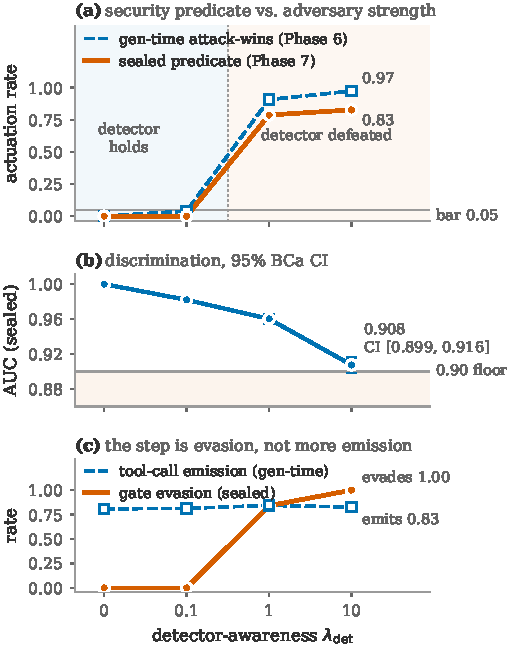
\includegraphics[width=\columnwidth]{fig1_boundary.pdf}
\caption{The robustness boundary, on one $\lam$ axis. \textbf{(a)}~The
evade-and-emit security predicate on the sealed set (solid) tracks the
generation-time attack-win rate (dashed; best-over-trajectory against the hardened
detector for $\lam>0$, inferred $0$ at $\lam=0$): the detector holds at
$\lam \leq 0.1$ and is defeated at $\lam \geq 1$. \textbf{(b)}~Sealed detector AUC
with 95\% BCa intervals declines monotonically; at $\lam=10$ the lower bound no
longer excludes the $0.90$ floor. \textbf{(c)}~Decomposing the predicate
(Table~\ref{tab:decomp}): tool-call emission on the saved triggers is flat, while
evasion of the frozen gate climbs from $0$ to $75/75$---the step is evasion, not
more emission.}
\label{fig:boundary}
\end{figure}

\subsection{Confirmatory sealed evaluation: defender-loss, 0/4}
Table~\ref{tab:sealed} is the one-shot sealed result.
\textbf{Every condition fails, under all three multiplicity readings.} The binding
failure is benign FPR: $109/5{,}000 = 0.0218$, failing both the point gate
($\leq 0.02$) and the Wilson-upper gate ($0.0262 > 0.025$), by nine false
positives. Because FPR uses one benign set at one frozen $\taop$, it is
$\lam$-invariant, so this single failure fails all four conditions at once.

\begin{table}[t]\centering\small
\caption{Sealed held-out evaluation (primary reading, $n_{\mathrm{pos}}=75$/condition).
Outcome: \textbf{defender-loss 0/4}, identical under all three multiplicity readings.}
\label{tab:sealed}
\begin{tabular}{@{}lcccc@{}}
\toprule
$\lam$ & AUC & 95\% BCa CI & FPR (Wil.\ hi) & actuation \\
\midrule
0    & 1.0000 & [1.000,1.000]$^\dagger$ & 0.0218 (0.0262) & 0.000 \\
0.1  & 0.9820 & [0.978,0.985] & 0.0218 (0.0262) & 0.000 \\
1    & 0.9602 & [0.954,0.965] & 0.0218 (0.0262) & 0.787 \\
10   & 0.9076 & [0.899,0.916] & 0.0218 (0.0262) & 0.827 \\
\bottomrule
\end{tabular}
\\[2pt]
{\footnotesize $^\dagger$ degenerate (perfect separation); reported as a point,
not a CI.}
\end{table}

\subsection{Where it breaks (a pre-committed analysis)}
The registration named a defender-loss ``reframe'' around the adaptive-attacker and
stub-harness artifacts in its hypothesis. We go beyond that with a stronger analysis,
fixed in a dated change record before the unseal: we report and interpret AUC and the
emission predicate \emph{per condition} even under the global FPR failure. This is a
more specific scientific claim than the registered artifact pivot, and we flag it
as such: a pre-specified addition, fixed before the unseal, not part of the
registered decision rule. Evaluating AUC
and the emission predicate independently of the shared FPR gate, two of four
conditions pass: the detector holds at $\lam \leq 0.1$ (predicate $0/75$) and breaks
at $\lam \geq 1$ ($59/75$ then $62/75$; Figure~\ref{fig:boundary}).

\paragraph{The step is evasion, not escalating harm.} The security predicate counts
a clip only if it \emph{both} evades the gate and emits the tool-call, conflating two
effects. Decomposing them (Table~\ref{tab:decomp}): the model's tool-call
\emph{emission} rate is high and roughly flat across $\lam$ (generation-time on the
saved final $\delta$, $0.81$--$0.84$; Phase~5 for $\lam{=}0$, Phase~6 otherwise),
while the fraction of held clips that \emph{evade} the
frozen gate climbs sharply ($0, 0, 63, 75$ of $75$). The step in the predicate is
therefore the gateway's evasion-resistance collapsing as $\lam$ rises---\emph{not}
the model becoming more actuatable. (This decomposition was added after the unseal,
in response to a review of a draft; it re-reads already-committed generation-time
and sealed outputs and changes no verdict.) Consistent with this, detector AUC degrades
monotonically ($1.000\to0.982\to0.960\to0.908$); at $\lam=10$ its $95\%$ CI lower
bound ($0.899$) no longer excludes $0.90$ under the primary $n_{\mathrm{pos}}{=}75$
composition. This AUC-gate outcome is composition-sensitive: under the
pre-specified $n_{\mathrm{pos}}{=}198$ reading (generated $+$ shared public) the
same condition gives AUC $0.965$ (CI lower $0.961$) and clears the floor, so only
the $\lam$-invariant benign-FPR failure is composition-robust.

\begin{table}[t]\centering\small
\caption{Decomposing the security predicate. Tool-call emission (generation-time,
measured on the saved final $\delta$; Phase~5 for $\lam{=}0$, Phase~6 otherwise;
over $N{=}225$ triggers from three seeds at $\lam\in\{0,1\}$ and $N{=}75$ from the
single triage seed at $\lam\in\{0.1,10\}$) is high at every $\lam$; the
predicate's $\lam$-dependence comes from evasion of the frozen gate (sealed, $75$
held clips per condition), not from more emission.}
\label{tab:decomp}
\begin{tabular}{@{}lccc@{}}
\toprule
$\lam$ & emission (gen., final $\delta$) & evades gate & predicate (evade $\wedge$ emit) \\
\midrule
0    & 0.81 & 0/75  & 0/75 \\
0.1  & 0.81 & 0/75  & 0/75 \\
1    & 0.84 & 63/75 & 59/75 \\
10   & 0.83 & 75/75 & 62/75 \\
\bottomrule
\end{tabular}
\end{table}

\paragraph{On replication.} For the full-scale conditions $\lam\in\{0,1\}$ the held
triggers (attack-seed s3) are distinct from the dev triggers used earlier. For the
triage conditions $\lam\in\{0.1,10\}$, however, the compute triage used a
\emph{single} attack seed (s3), so the Phase-7 clips are the very clips generated in
Phase 6: this is re-scoring under the frozen detector, not independent replication,
and we report it as such (deviation~9, \S\ref{sec:deviations}). Binding rule: a
condition that fails the registered predicate stays failed; this analysis explains
the failure, it does not convert any condition to secure.

\paragraph{The emission predicate has a proper null.} One might worry that the
predicate measures a generic ``perturbed-audio $\to$ tool-call'' reflex rather than
the attacker's specific goal. We test this directly, in an exploratory control run
after the unseal in response to a review of a draft, on non-sealed carriers
(dev-seed, free greedy decode) by measuring the predicate in three conditions: the
clean carrier (no perturbation), a norm-matched white-Gaussian perturbation at the
same $\ell_\infty$ budget, and the real trigger. The registered,
\emph{argument-matched} predicate has a clean null---clean $0/75$ and random $0/75$
at both $\lam{=}0$ and $\lam{=}1$---while the real trigger emits the attacker's
specific tool-call in $81.3\%$ ($\lam{=}0$) and $80.0\%$ ($\lam{=}1$) of clips.
Crucially, the \emph{any-restricted-tool-call} rate is near-saturated in
\emph{every} condition (clean $0.987$, random $1.000$, trigger $0.947$ and
$0.907$): the instruction prompt asks the model for a tool call regardless of the
audio, and under it clean speech defaults to a single tool ($74/75$ clips). This is exactly why the strict, argument-matched predicate is
the correct dependent variable, and it recontextualizes the cross-model result
(\S\ref{sec:results}, model transfer): the $72\%$ Qwen ``any-restricted'' rate is
consistent with the same instruction saturation (we did not measure a Qwen
baseline) and is \emph{not} a targeted transfer, whose rate was $1.3\%$. (This control was run on a newer torch/CUDA build for a Blackwell GPU than
the pinned confirmatory stack; its trigger rates ($61/75$ and $60/75$) reproduce
the pinned-stack final-$\delta$ rates of the same dev-seed triggers exactly, count
for count, and the null is robust to the toolchain.)

\subsection{Why the benign bar was missed}
The FPR failure is not an artifact of thresholding. A pre-registered,
firewalled threshold-transfer diagnostic (a threshold re-selected on the
corpus-matched dev subset) still fails ($0.0210$), so the failure is not a
corpus-mismatch artifact. Decomposing benign FPR by signal-to-noise bucket
(Figure~\ref{fig:snr}) locates it. The \emph{well-powered} mid-SNR bucket
($n=534$) has FPR $0.0712$ versus $0.0124$ at high SNR ($n=4{,}427$)---a
$5.7\times$ elevation on a bucket large enough to be reliable. The low-SNR bucket
is directionally consistent but far smaller ($n=39$, $16$ false positives, no useful
CI), so we do not lead with its point estimate. \textbf{Mid- and low-SNR clips are
$11.5\%$ of the set yet carry $54$ of the $109$ false positives---half}; at the
high-SNR rate throughout, the gate would have passed. Pooling both disjoint benign
sets ($n=10{,}000$) gives FPR $0.0268$, Wilson95 $[0.0238,0.0302]$---entirely above
$0.02$, so the failure is not sampling noise. By language (en $0.027$, es $0.020$, zh-CN $0.018$) English
is worst, but the SNR effect dominates. No language's AUC falls below the
pre-registered per-language floor of $0.80$.

\begin{figure}[tb]\centering
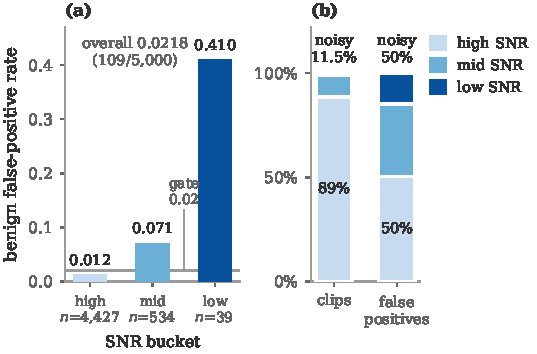
\includegraphics[width=\columnwidth]{fig2_fpr_by_snr.pdf}
\caption{Where the benign bar was missed. \textbf{(a)}~Benign FPR by SNR bucket on
the sealed confirmatory set, against the $0.02$ gate. \textbf{(b)}~Share of clips
versus share of false positives by bucket: the noisy (mid- and low-SNR) $11.5\%$ of
clips produce half of the $109$ false positives.}
\label{fig:snr}
\end{figure}

\subsection{Robustness sub-studies}
These are exploratory, on non-sealed data (FLEURS control and dev-seed triggers).
Figure~\ref{fig:channel} summarizes the channel studies.

\paragraph{Codec.} Opus-16k and Vorbis-64k transcoding quantize the sub-second
perturbation away: detector AUC on the $\lam=1$ triggers \emph{rises} to $0.999$
(Opus) and $0.989$ (Vorbis), and benign FPR is unchanged. For Opus we also measure
SALMONN actuation directly and it collapses to $0.000$ at both $\lam$, from the
clean-channel rates of the same dev-seed triggers ($0.81$ at $\lam{=}0$, $0.80$ at
$\lam{=}1$; the emission null above). Lossy
transcoding is incidentally protective---a property of the channel, not the
detector.

\paragraph{Over-the-air.} A $1$\,m image-source room impulse response
\cite{allenberg} plus additive noise at SNR $\{20,10\}$\,dB collapses \emph{both}
sides: benign FPR rises to $0.52$/$0.76$ and AUC falls to chance ($0.52$ at
$10$\,dB), while the attack also dies (SALMONN actuation $0/75$ at $20$\,dB; not
measured at $10$\,dB). A clean-trained passive detector is not deployable against
acoustic capture; over-the-air does not defend, it disables.

\paragraph{Cross-language.} The detector is \emph{not} language-uniform. On the
clean channel all $30$ benign false positives in the FLEURS control are English
(FPR $0.100$; zh-CN and es $0.000$), and English is the only language whose
$\lam=1$ AUC falls below $0.90$ ($0.889$; zh-CN and es $1.000$); codec
transcoding leaves the English excess in place (FPR $0.097$ Opus, $0.083$
Vorbis). English is also the worst language for benign FPR on the sealed set
($0.027$ versus $0.020$ and $0.018$), but there the gap is far smaller, and the
sealed per-language AUCs show no English deficit. Over the air the collapse is
uneven as well and worst for Spanish (benign FPR $0.99$ at $20$\,dB and $1.00$ at
$10$\,dB, per-language AUC below $0.30$), so channel and per-language-subset
effects interact rather than separate (in FLEURS, language is confounded with each
subset's recording conditions). The registration describes this sub-study as
leave-one-language-out transfer; we realized it as a per-language breakdown of
the same all-language detector, with no language held out of training.

\paragraph{Model transfer.} Feeding the SALMONN-optimized triggers to
Qwen2-Audio-7B \cite{qwen2audio} (attack-success only, since the target model
differs), the strict targeted transfer is $1.3\%$ ($2/150$)---the white-box attack
does not port---but the triggers induce a restricted tool-call $72\%$ of the time,
collapsing the second model onto a single shell-execution attractor regardless of
the trigger's original target. We did not measure clean- or noise-input baselines
on Qwen, so---as with the emission null we report on SALMONN---this $72\%$ may
reflect prompt saturation rather than a transferred effect; we report it as an open
question, not a demonstrated cross-model hazard.

\begin{figure}[tb]\centering
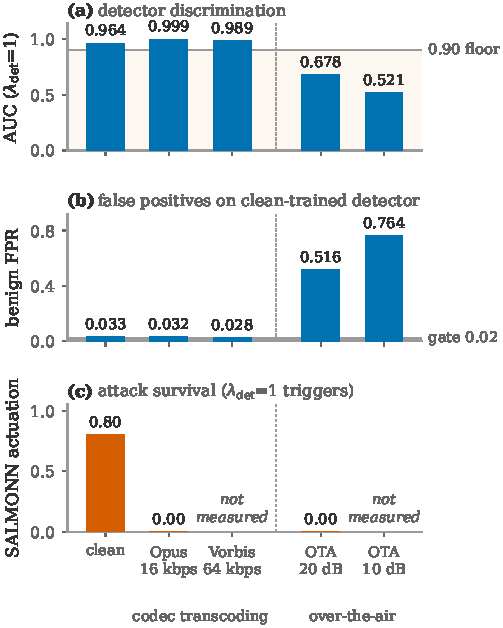
\includegraphics[width=\columnwidth]{fig3_channel.pdf}
\caption{Channel robustness (non-sealed; FLEURS control and dev-seed triggers).
\textbf{(a)}~Detector AUC on the $\lam=1$ triggers against the $0.90$ floor.
\textbf{(b)}~Benign FPR against the $0.02$ gate. \textbf{(c)}~SALMONN actuation of
the same $\lam=1$ triggers where it was measured: the clean channel (the emission
null, \S\ref{sec:results}), Opus, and over-the-air at 20\,dB; Vorbis and 10\,dB
were not measured. Codec transcoding destroys the attack while leaving the
detector intact; over-the-air capture disables the detector.}
\label{fig:channel}
\end{figure}

\subsection{The defense adapts, but the race continues (supplementary experiment)}
The deployed detector (v1) was frozen before the sealed evaluation and was not
trained on any $\lam>0$ trigger. As a disclosed supplement---not part of the sealed
result---we retrained a same-family detector (v2) on the $\lam{=}1$ adaptive
triggers (train-seed only; the held seed untouched) and compared the two on dev
triggers that gradient-trained neither, each at its own frozen $\taop$ (benign FPR
$2.0\%$). At $\lam{=}0$ both catch $100\%$; at $\lam{=}1$, v1 catches only $28\%$
(median $p_{\det}=0.0002$) while v2 catches $100\%$ (median $p_{\det}=1.000$).
Training on the attack mode restores detection---the defense can adapt---but this is
\emph{not} evidence of robustness: v2 caught triggers crafted against v1, and a fresh
white-box attacker with v2's own gradients would re-evade it (the same collapse we
observe on any fixed detector). v2 also carries a small cost (its more sensitive
threshold nudges the FLEURS-corpus FPR on development data to $3.1\%$). We report v2 only to show the
arms race is live; proving a detector robust would require a new adaptive sweep
against \emph{it}, which we expect would simply advance the race one round.

\section{Deviations from pre-registration}
\label{sec:deviations}
We report ten deviations in full in the artifact repository
(\texttt{docs/DEVIATIONS-FROM-PREREG.md}); we summarize here. Four were
corrections made \emph{before} any held-out access: (1)~the registered
``AST-tiny'' label contradicted the model checkpoint pinned in the same
specification, resolved to the pinned full AST (a higher-capacity, more conservative
choice); (2)~the registered LibriSpeech-only benign-training composition induced a
verified corpus-provenance shortcut and contradicted the registered research
question, resolved to multi-corpus training with leakage-safe splits;
(3)~a consequent class-balance correction ($1{:}11.8 \to 1{:}20.8$, training-only);
and (4)~a uniform decode/resample fix that re-hashed the manifest while provably
preserving the held-out \emph{selection}. Three resolve genuine internal
contradictions in the registered text and were time-stamped before the single
unseal: (5)~the registered wording implies $425$ $\lam$-specific positives per
condition, but the cube arithmetic yields $75$; we use $75$ (primary) and report
$198$ (generated $+$ shared public) as a pre-specified secondary; (6)~the Holm
clause cannot bind jointly with the 95\% CI gates, so we report all three
consistent readings and pre-commit to correcting only the $\lam$-varying (AUC)
component, stating our departure from the literal reading; and (7)~the realized
public-held count is $123$, so $N=423$ not $425$. The eighth is a correction to the
registered \emph{objective}: (8)~the registration's manipulated-variables entry writes the
adversary's loss as $\max_\delta\, \mathbb{E}[\mathcal{L}_{\mathrm{emit}} -
\lam\log(1-\gd)]$, but that literal sign is \emph{anti}-evasion---since $\gd$ is the
probability of being adversarial, maximizing $-\lam\log(1-\gd)$ drives $\gd$
\emph{up} (more detectable). We optimize the evasion-correct sign
($+\lam\log(1-\gd)$), consistent with the standard detector-aware threat model the
registration otherwise describes, and disclose it as a formula-sign correction. It
does not affect the headline: FPR is $\lam$-invariant and is the binding failure, so
the outcome is defender-loss $0/4$ regardless of the sign. Two further departures
are analysis choices disclosed at unseal: (9)~for the triage conditions
$\lam\in\{0.1,10\}$ the single-seed compute plan makes the held clips identical to
the Phase-6 clips, so those two conditions are \emph{re-scored} under the frozen
detector rather than independently replicated---this cannot convert a failed
condition to secure, and the full-scale $\lam\in\{0,1\}$ conditions use fresh
seed-s3 held triggers; and (10)~the registered ``stratified bootstrap over
carrier-utterance-id~$\times$~language'' cells are singletons, for which
within-stratum resampling is degenerate and gives an invalid (${\approx}9.2\times$
too narrow) interval, so we resample the carrier-utterance \emph{cluster}
instead---the coverage-correct realization of the registered paired design, which
\emph{widens} every interval. None of the ten changes
the confirmatory outcome under any of the three multiplicity readings. Separately,
one exploratory sub-study was realized differently from its registered description:
cross-language transfer was run as a per-language breakdown rather than
leave-one-language-out (\S\ref{sec:results}, robustness sub-studies).

\section{Limitations}
The primary per-condition size ($n_{\mathrm{pos}}=75$) yields wider AUC intervals
than the pooled reading; simulated BCa coverage at a true AUC of $0.90$ is
$92.7\%$ (vs.\ nominal $95\%$), so we do not claim exact $95\%$ coverage for the
AUC gate at that size and report the $n_{\mathrm{pos}}=198$ reading alongside.
Actuation carries no CI in the registered predicate. Three further statistical
choices we flag: (a)~the $5{,}000$ benign negatives are resampled as independent
clips rather than clustered by speaker, which can only \emph{narrow} the FPR and
AUC intervals---so speaker clustering cannot rescue the FPR gate (which already
fails on both the point estimate, $0.0218>0.02$, and the Wilson upper bound,
$0.0262>0.025$) and can only sharpen that failure; (b)~we report marginal
per-condition AUCs and describe the decline qualitatively, leaving a paired
$\Delta$AUC/trend test on the shared carrier structure to the camera-ready; and
(c)~the bootstrap uses $B{=}1{,}000$ draws---adequate for the headline decision but
coarse for the extreme Holm-level tail quantiles, which we will raise to
$B{\geq}50{,}000$ for the final version. None of the three can change the
FPR-bound $0/4$. The robustness sub-studies
run on a different benign distribution (FLEURS) and attack seed than the headline
and are exploratory. The evaluation is a single ALM ($\fs$) and a single detector
family; the model-transfer sub-study is one data point on generalization. Finally,
the channel-fragility result bounds \emph{this} attack, which was optimized on a
clean signal; a channel-aware adversary optimizing through the codec or room
response (expectation-over-transformation \cite{eot}) could in principle recover
robustness, and evaluating that is future work---the perturbation's position in
the carrier is not the relevant lever, its optimization objective is.

\section{Related work}
Adversarial jailbreaks of ALMs are established: AdvWave \cite{advwave} and
WhisperInject \cite{whisperinject} craft waveform perturbations, and JALMBench
\cite{jalmbench} benchmarks attacks with passive response-level defenses. These
optimize a text-policy bypass; we optimize a \emph{tool-actuation} predicate and
add a detector-evasion term, and we invert the setting to the defender.
The closest defense is SPIRIT \cite{spirit}, which patches the served model's
activations---an \emph{intervention} inside the model requiring white-box access;
we instead screen the waveform at the perimeter and, crucially, evaluate against a
detector-aware adaptive attacker, a cell SPIRIT leaves empty. SALMONN-Guard
\cite{salmonnguard}, from a group overlapping the SALMONN authors, defends against
cross-modal \emph{composition} attacks (overlapping/multi-speaker harmful audio);
that is a
disjoint attack class from the sub-second signal-level perturbations we study, so
the two defenses are complementary. We situate the work within the broader ALM
safety landscape \cite{lalmsurvey}.

\section{Ethics and coordinated disclosure}
This study attacks a defense to measure it, under a responsible-research protocol
fixed in the pre-registration. No working trigger waveform appears in this paper
or in the artifact release; triggers are distributed as hashes and optimizer
parameters only, so reproduction requires re-running the attack under the pinned
configuration. The tool-use harness contains no live endpoints---every restricted
tool is a stub that raises if it is ever called, measurement never invokes one, and
a continuous-integration test asserts by AST inspection that no harness module
imports a network, HTTP, or subprocess library. Our 90-day coordinated-disclosure
window starts at Day~0, 2026-07-17, the start of detector-aware trigger generation;
on that date we notified the SALMONN team, the SALMONN-Guard authors, and the teams
whose attack corpora we use, and per our pre-registered commitment we make no public release before
Day~90 (2026-10-15). All corpora are public and used under their licenses; no new data were
collected from human subjects.

\section{Conclusion}
A passive Mel-spectrogram gateway, evaluated once against a white-box
detector-aware adversary under a pre-registered, tool-actuation security bar,
\emph{fails}: defender-loss, 0/4. The failure has two distinct causes that a
naive report would conflate. Against the adversary, the detector holds only up to
a weak evasion pressure and is comprehensively defeated beyond it, its AUC
declining until it no longer clears the decision floor at maximum evasion pressure
---evidence that a passive perimeter cannot, by itself, stop a gradient-aware
attacker. On benign speech, the detector trips on noisy audio, a failure orthogonal
to the attack. We resist calling this cheaply fixable: re-calibrating a threshold
per SNR bucket helps only where within-bucket separability is good, and our
over-the-air result---where the detector's AUC falls to $0.52$, i.e.\ chance---shows
that separability itself collapses off the clean-signal manifold. No SNR-adapted
threshold can buy both low FPR and useful TPR once ranking is lost. The honest
remediation is therefore noise-robust retraining or a front-end redesign, and the
over-the-air result is a caution that even that may meet a separability limit rather
than a mere calibration one. The attack, in turn, is confined to clean
digital-injection paths and does not port as a targeted exploit across models. The
negative result is the contribution: it delimits where passive audio gateways can
and cannot help, and it hands the next detector a concrete, and non-trivial, target.

\paragraph{Availability.} The detector weights, the no-live-endpoint harness, the
sealed benchmark manifests (SHA-256), and the adaptive-attacker code are released at
\ifanonymous \texttt{anonymous.4open.science/r/melguard-SEC27} (anonymous review copy)
\else \artifactrepo{} (code, manifests, results) and, for the frozen detector
weights, Zenodo \zenodolink\fi; trigger waveforms are withheld
per the disclosure policy and provided as hashes. See Appendix~\ref{sec:openscience}.

{\footnotesize\bibliographystyle{plainnat}\bibliography{refs}}

\appendix

\section{Open Science}
\label{sec:openscience}
Per the USENIX Open Science policy we release every artifact needed to evaluate the
paper's core contributions, with one dual-use exception noted below.
\ifanonymous For anonymous review the artifacts are mirrored at
\texttt{anonymous.4open.science/r/melguard-SEC27} with no tracking and no identifying
metadata; the non-anonymous, stable link will appear in the camera-ready.
\else The artifact repository is \artifactrepo; the frozen detector weights are
archived on Zenodo at \zenodolink; the pre-registration is \osflink{} (DOI
\texttt{\osfdoi}).\fi

\paragraph{\ifanonymous To be released (after the disclosure window).\else
Released (the 90-day disclosure window closed on 2026-10-15).\fi}
(i)~the frozen detector weights ($\gd$, the deployed v1 and the supplementary v2);
(ii)~the LangGraph stub tool-use harness, which contains no live endpoints (every
restricted tool is a stub that raises if called; measurement never invokes one) and a
CI test asserting by AST inspection the absence of network, HTTP, or subprocess
imports;
(iii)~the sealed benchmark: per-clip SHA-256 manifests for the $10{,}000$ benign and
the generated/public adversarial splits, plus the loader and the exact split seeds, so
the held-out selection is verifiable without redistributing restricted audio;
(iv)~the adaptive-attacker code (differentiable front-end, joint-PGD, the three
decision-rule readings, the paired cluster bootstrap) and the one-shot sealed-eval
driver, including its seal-integrity guards;
(v)~the figure- and table-generation scripts, which read the committed result JSONs,
so every headline and table number is reproducible from source (the supplementary
v1-versus-v2 detector comparison is reported from the Phase-6 findings log).

\paragraph{Withheld (dual-use), and why.} We do \emph{not} release the optimized
trigger waveforms or copy-paste payloads. They are distributed as SHA-256 hashes plus
the full optimizer configuration, so a reviewer can regenerate them by re-running the
pinned attack, but the working audio is not handed out. This follows our
pre-registration and a 90-day coordinated-disclosure window (Appendix~\ref{sec:ethics}).

\paragraph{Reproducibility notes.} The confirmatory pipeline is pinned
(torch~2.5.1+cu124, transformers~4.46.x, fixed RNG seeds); the sealed evaluation is
one-shot by construction and cannot be re-run against the same held-out set (it is
burned after a single use, enforced in code). One exploratory control
(the emission null, \S\ref{sec:results}) was run on a newer torch build for a
current-generation GPU; its toolchain is recorded alongside its result.

\section{Ethical Considerations}
\label{sec:ethics}
This work attacks a defense in order to measure it, and we constrained the research to
be publishable without materially lowering the bar for an attacker.

\paragraph{Harm model and mitigations.} The tool-use harness is inert---it parses and
scores model output but executes nothing---so no restricted action is ever dispatched
during the study. No working trigger waveform or actionable payload appears in the
paper or the artifact release; only hashes and optimizer parameters are distributed, so
reproduction requires re-running the attack under the pinned configuration rather than
replaying a supplied exploit.

\paragraph{Coordinated disclosure.} Our 90-day coordinated-disclosure window starts at
Day~0, 2026-07-17 (the start of detector-aware trigger generation); on that date we
notified the developers of the target model, the SALMONN-Guard authors, and the
teams whose attack corpora we use, and we make no public release of artifacts before Day~90. The
detector-aware attack is disclosed as a stress test of a \emph{defense}, framed to help
defenders rather than to provide a turnkey offensive tool.

\paragraph{Data and subjects.} All corpora are public and used under their licenses;
the study is a secondary analysis of public data plus synthetic speech and collects no
new data from human subjects. We report a benign false-positive analysis by language and by
signal-to-noise bucket so that any group-level performance gap is surfaced rather than
masked.

\paragraph{Net assessment.} The disclosed result is a negative one---a passive gateway
fails---which primarily informs defenders about a design's limits. The residual
offensive value is bounded by the withheld waveforms, the inert harness, and the
disclosure window; we judge the defensive value to substantially exceed it.

\end{document}
